\chapter {Planning with OMPL}
\label {chp:ompl}

The Open Motion Planning Library provides an abstract representation for all
of the core concepts in motion planning, including the state space, control space,
state validity, sampling, goal representations, and planners.  This chapter
discusses OMPL and how its components relate to the ideas from the motion
planning literature.  The first section discusses the design considerations of
the library.  The second section maps the components of OMPL to their logical
equivalents in the motion planning literature.  The third elaborates on the
use of OMPL for solving motion planning queries using sampling-based techniques
composed from the objects described in Chapter \ref{chp:motionplanning}.  The
fourth section details the compilation of code written using OMPL, and the final
discusses OMPL's benchmarking capabilities.

There exists a wide variety of documentation, tutorials, and other examples
regarding the use of OMPL at {\tt ompl.kavrakilab.org}.  Specifically, the
website has extensive resources for installation, hands-on tutorials, as well
as the API documentation.  Additionally, a group exists at {\tt sourceforge.net}
called ``ompl-users'', which contains a forum for posting comments, questions,
and bug reports.

\section {Design Considerations}
\label{chp:design}
OMPL is flexible and applicable to a wide variety of robotic systems.  As a
consequence to this flexibility, the library does not explicitly represent the
geometry of the workspace or the robot operating in it.  This is deliberate
since there exists a vast amount of file formats, data structures and other
means of representation for robotic systems.  As a result, the user must select
a computational representation for the robot and provide an explicit state
validity/collision detection method.  There does not exist a default collision
checker in OMPL.  This allows the library to operate with relatively few
assumptions, allowing it to plan for a huge number of systems while remaining
compact and portable.

A conscious effort is also made to limit the number of external dependencies
necessary to compile and execute the code in OMPL.  The majority of the third
party code utilized in the library used comes from Boost \cite{Boost}, which
allows OMPL to function in most major operating systems.  Currently, OMPL is
supported on Linux and Mac OS X.  Windows installation of the core OMPL
library is also possible by compiling from source.  Installation of OMPL.app on
Windows can also be done, but this is recommended only for experienced Windows
developers as the installation of the dependencies is challenging.

\section {OMPL Foundations}
Chapter \ref{chp:motionplanning} showed that many sampling-based motion planners
require a few similar components to solve a planning query: a sampler to compute
valid configurations of the robot, a state validity checker to quickly evaluate
a specific robot configuration, and a local planner to connect two samples along
a collision free path.  OMPL provides most of these components in similarly
named classes.  The following OMPL classes are analogous to ideas in traditional
sampling-based motion planners:

\paragraph {StateSampler} The StateSampler class implemented in OMPL
provides methods for uniform and Gaussian sampling in the most common state
space configurations.  Included in the library are methods for sampling
in Euclidean spaces, the space of 2D and 3D rotations, and any combination
thereof with the CompoundStateSampler.  The ValidStateSampler takes advantage
of the StateValidityChecker to find valid state space configurations.

\paragraph {StateValidityChecker} The StateValidityChecker is tasked with
evaluating a single state to determine if the configuration collides with an
environment obstacle and respects the constraints of the robot.  A default
checker is \emph{not} provided by OMPL for reasons stated in Section
\ref{chp:design}.  Since this component is an integral part of sampling-based
motion planning it is necessary for the user to provide the planner a callback
to such a method to ensure that all configurations are feasible for the robot.

\paragraph {NearestNeighbors} This is an abstract class that is utilized
to provide a common interface to the planners for the purpose of performing a
nearest neighbor search among samples in the state space.  The core library
has several types of nearest neighbor search strategies at its disposal,
including Geometric Near-neighbor Access Trees (GNATs)~\cite{Brin:1995}
and linear searches.
It is also possible to use an external data structure and supply the core library
with this implementation.

\paragraph {MotionValidator} The MotionValidator class (analogous to the local
planner) checks to see if the motion of the robot between two states is valid.
At a high level, the MotionValidator must be able to evaluate whether the motion
between two states is collision free and respects all the motion constraints of
the robot.  OMPL contains the DiscreteMotionValidator, which uses the
interpolated movements between two states (computed by the StateSpace) to
determine if a particular motion is valid. This is an approximate computation as only a finite number of states along the motion are checked for validity (using the StateValidityChecker).

\paragraph {ProblemDefinition} A motion planning query is specified by the
ProblemDefinition object.  Instances of this class define a start state and goal
configuration for the robot.  The goal can be a single configuration or a region
surrounding a particular state.

\section {Solving a Query}
The previous set of objects are just a subset of the classes used in OMPL.
Figure \ref{fig:ompl:hierarchy} shows the hierarchy of the major components
of OMPL and how they are interrelated.

\begin {figure}[h]
\centering
{
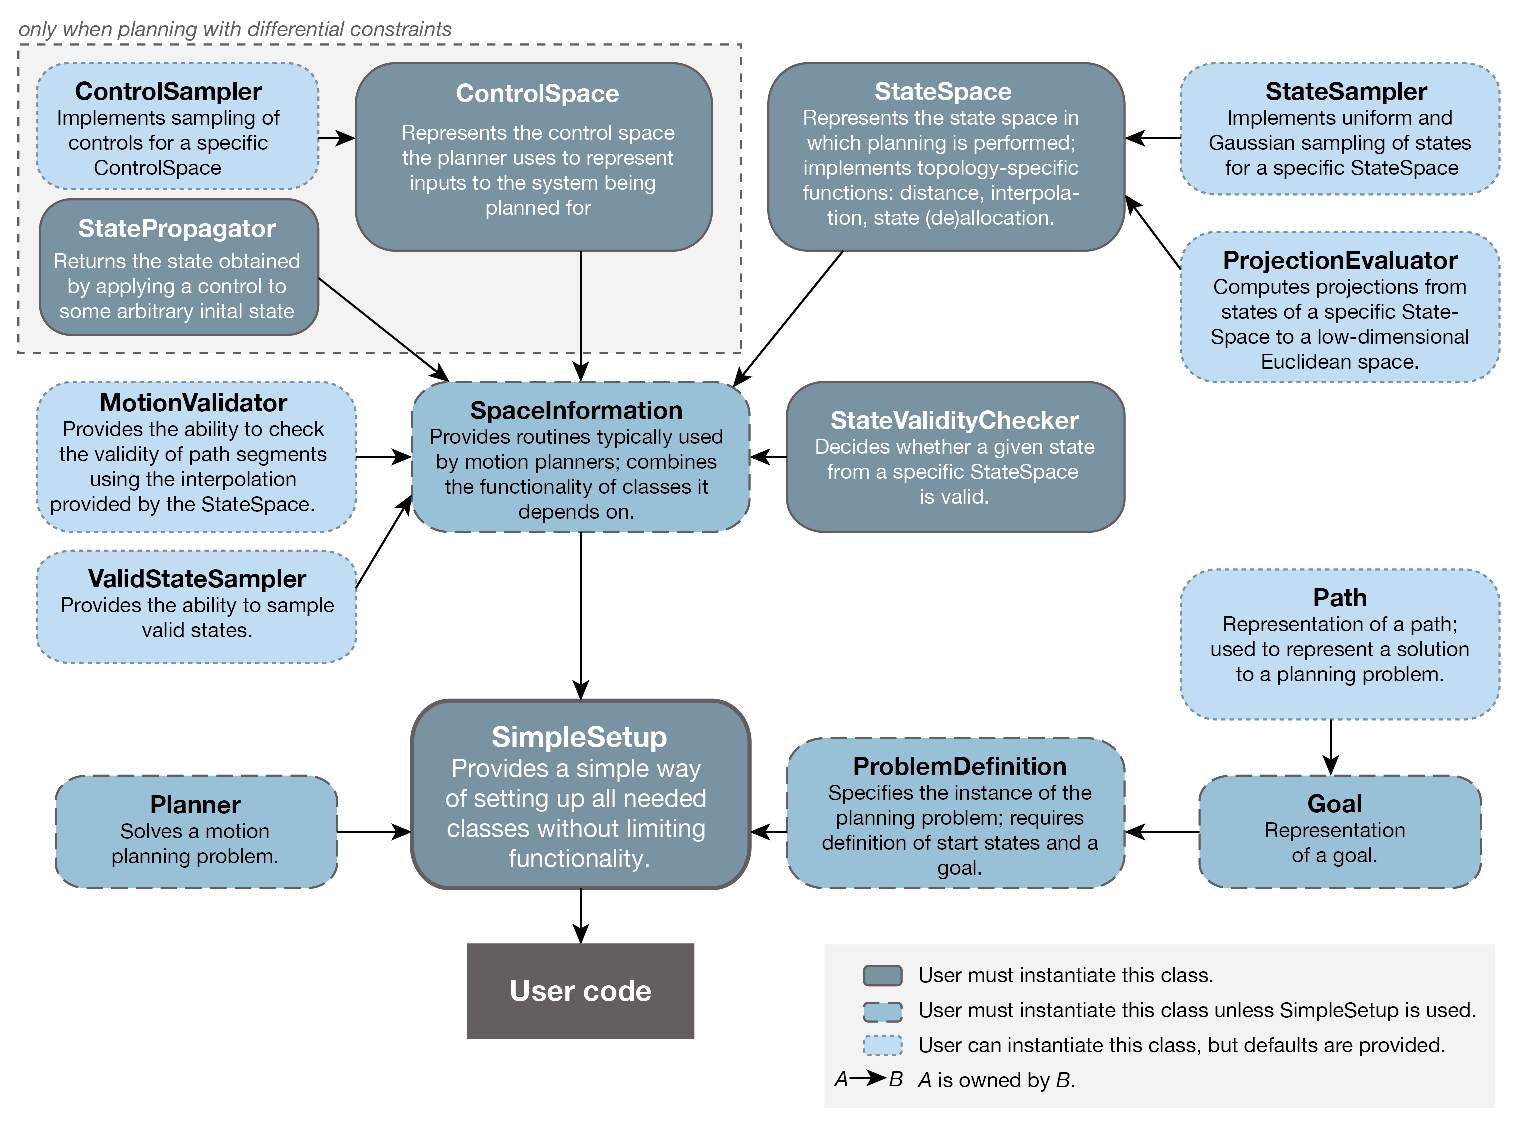
\includegraphics [width=.9\textwidth]{ompl_hierarchy}
\caption {The hierarchy of the high level components of OMPL.  Objects
highlighted in dark blue are required to be instantiated by the user.}
\label {fig:ompl:hierarchy}
}
\end {figure}

The object oriented nature of OMPL allows the user to inherit from currently
existing components or create brand new components to plan for a specific
system.  When solving a particular query, the user is not required to
instantiate all of the objects detailed in Figure \ref{fig:ompl:hierarchy}.
In fact, most of these objects have default implementations that are
sufficient for general planning.

\paragraph {Geometric Planning}
For geometric motion planning, the user must define and instantiate the state
space object for the robot, and provide a start and goal configuration in that
space to define the motion planning query.  Any planner defined in the
geometric namespace can then be employed to solve the motion planning query.

\paragraph {Planning with Controls}
Like geometric planning, when planning with controls the user must define and
instantiate the state space for the robot, and provide a start and goal
configuration.  In addition, the user must define valid control inputs via
a ControlSpace object, and provide a method for computing how the system state
changes when applying valid controls using a StatePropagator instance.  The
user can use any planner in the control namespace to compute a solution.

\paragraph {SimpleSetup}
SimpleSetup provides a way to encapsulate the various objects necessary to
solve a geometric or control query in OMPL.  When using SimpleSetup, the user
only supplies the state space, start state, and goal state (and state propagator
for planning with controls). Specifically, SimpleSetup instantiates the
SpaceInformation, ProblemDefinition, and Goal objects.  Additionally,
SimpleSetup allows for the retrieval of all of these subcomponents for further
customization.  This means that SimpleSetup does not inhibit any native
functionality of OMPL, and ensures that all objects are properly created before
planning takes place.  Moreover, SimpleSetup exposes fundamental function
calls for ease of use.  For example, the function ``solve'' from the Planner
class is available in SimpleSetup, and it is not necessary for the user to
extract the Planner from the SimpleSetup instance to do so.

\section {Compiling Code with OMPL}
Once a new planner, sampler, collision checker, or other motion planning
component has been developed, it is simple to integrate with OMPL for testing.
There are two methods for compiling code with OMPL.  If the base library is
modified (e.g., a new planner is added to  {\tt ompl/geometric/planners}),
simply re-run \emph{cmake} to reconfigure the makefiles for that particular
component of the code.  If the new code does not exist in a directory known to
\emph{cmake}, {\tt ompl/src/ompl/CMakeLists.txt} will need to be updated to
search in the extra directory.

If OMPL has been installed, new code can be compiled independently from OMPL.
The core OMPL library can be linked into the final binaries using the
traditional linking step.  For example, if compiling with GCC, simply link the
code with ({\tt -lompl}), and direct the compiler to search the install
directory for the library.  A similar linking procedure can be employed
with other compilers.

\section {Benchmarking}
The ability to compare two or more planners has never been easier than with
OMPL.  OMPL provides a Benchmark class that attempts a specific query a given
number of times, and allows the user to try any number of planners.
Additionally, the Benchmark instance can be configured to fail an attempt after
a specific amount of time or when the planner exhausts a given amount of memory.

When the benchmarking has finished, the Benchmark instance will write a log
file to the current working directory containing information regarding every
planning attempt.  OMPL is packaged with a Python script to parse this log file
and create an SQL database with the planning information.  The Python script can
also query this database and generate a series of plots using matplotlib, like
those in Figure \ref {fig:benchmark:plot}.

\begin {figure}
\centering
{
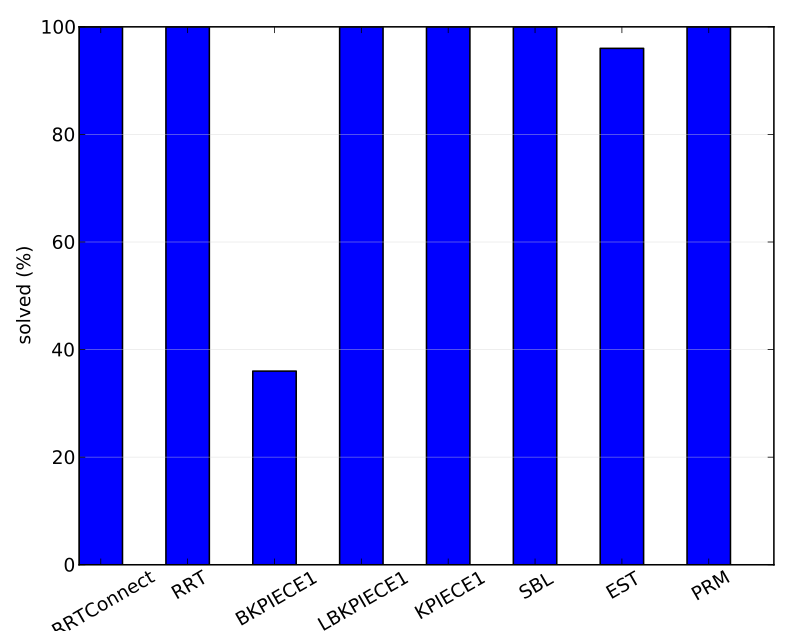
\includegraphics [width=3.75in]{twistycool_solved}\\ \vspace {0.25in}
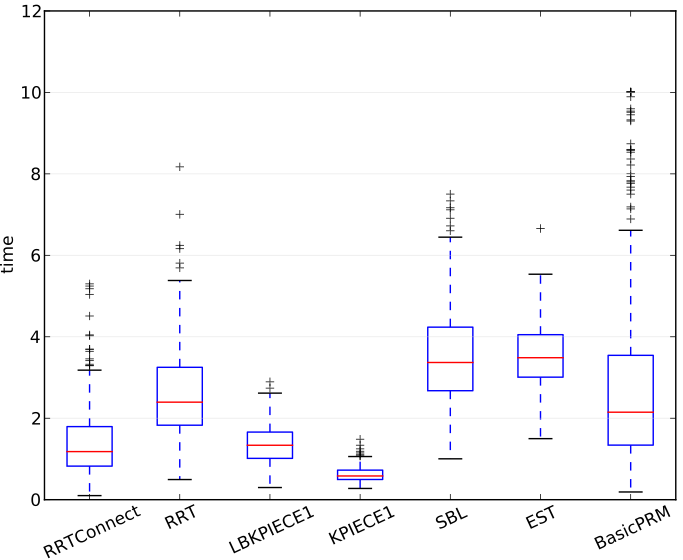
\includegraphics [width=3.75in]{cubicles_time}
\caption {Example benchmarking plots. (top) The percentage of instances solved by various
planners during one benchmark run. (bottom) A box plot showing the amount of time needed
for various planners to solve a planning instance}
\label {fig:benchmark:plot}
}
\end {figure}


